\documentclass[]{article}
% packages
\usepackage{../../cs70}
\usepackage{../../markup}
\usepackage{enumerate}
\usepackage{hyperref}
%% \usepackage{framed}
%% \usepackage{MnSymbol}
%% \usepackage{epstopdf}
\usepackage{color}
%% \usepackage[]{amsmath}
%% \usepackage{graphicx}
%% \usepackage{amssymb}
%% \usepackage{parskip}
%% \usepackage{rotating}
%% \usepackage{float}
%% \usepackage{multirow}
%% \usepackage{subcaption}
%% \usepackage{indentfirst}
%% \usepackage[left=1.5in, right=1.0in, top=1.0in, bottom=1.0in]{geometry}

\newif\ifsolutions
\newif\ifmotivation
\motivationtrue
\motivationfalse
\solutionstrue
%\solutionsfalse %flag for solutions

\renewcommand{\answer}[1]{{\color{mydarkblue}\textbf{Solution:}#1}}
\definecolor{mydarkblue}{rgb}{0,0.25,1}

\def\title{Homework 9}

\begin{document}

\maketitle
\config{hwnum}{6}
\config{homework-due}{03/31/2014 13:00}
\config{grades-due}{04/07/2014 13:00}
\vspace{0.5em}
{\Large{\textbf{This homework is due Mar 31 2014, at 12:00 noon.}}}

\begin{qunlist}
  
\qns{Virtual Lab 3: Biased Coins Continued}\\    
In this problem we will continue the lab from last HW. We will start from the optional problem at the end.
\begin{enumerate}[a)]
\qpart 
\item  Up till this point, everything that
  you have done in this virtual lab is something that you could've
  naturally discovered yourself as something worth trying. The data is
  speaking directly to the experimentalist in you. However,
  discovering an actual formula for the shape of this ``cliff-face'' is
  something that actually requires a theoretical investigation that is
  related to counting, Fourier Transforms, and Power Series. Guessing
  its exact shape is not something that comes very naturally on
  experimentalist intuition alone.

  So here, we will simply provide you with the right curve.

  Plot $\int_{-\infty}^d\frac{1}{\sqrt{2\pi}} e^{-\frac{x^2}{2}}dx$
  overlaid with the normalized cliff-face shapes you had plotted in
  the earlier parts. (Do this integral numerically or use the special
  functions that most numerical packages already have for computing
  these sorts of integrals. This integral is related to something
  called the Error Function.) Notice how beautifully it hits the exact
  shape. 

  This is the heart of the Central Limit Theorem as applied to coin
  tosses.

%\ifsolutions{ \answer { \\
%Suggestions for python students: check out the "math.erf()" and investigate its relationship with the normal CDF.
%\begin{figure}[h!]
%\center
%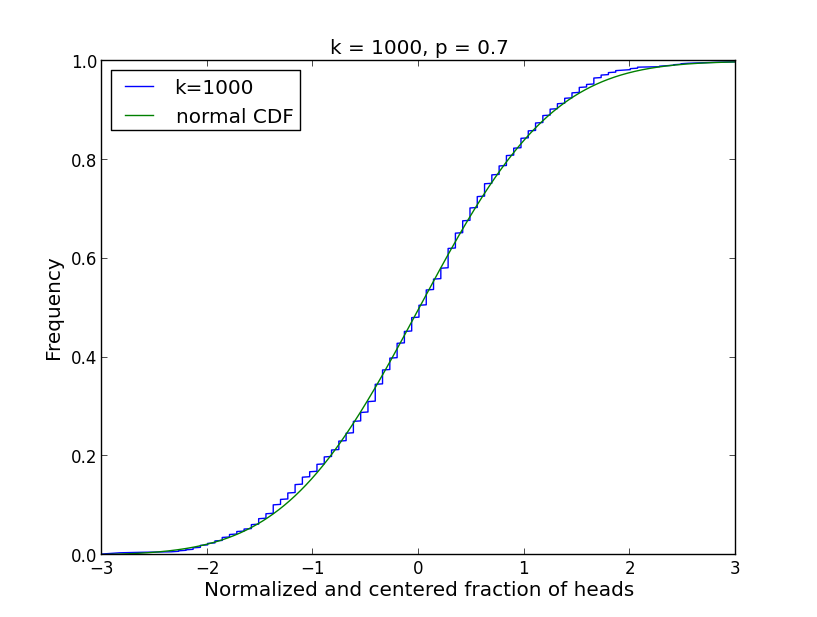
\includegraphics[width=0.45\textwidth]{figs/part_a.png}
%\end{figure}
%}}\fi

\qpart
\item Just a little notation. We will use $X_i$ to denote a random
  variable that is 1 if you toss a head on the $i$-th toss, and 0 if you toss a
  tail on the $i$-th toss. (This is just so we can more easily express 
  things) So a sequence of $k$ coin tosses would be $X_1, X_2, \ldots,
  X_{k-1}, X_k$, with each $X_i$ being 0 or 1 depending on how the run
  actually came out. How would you write the total number $S$ of heads
  as a function of the $X_i$'s? 

 Our experience from the last homework tells us that the total number
 of heads is itself a random quantity since it varies based on the
 vagaries of the coin tosses.


\qpart 
\item Now, since you had realized earlier that the cliff-faces and the
  histograms have some natural relationship with each other, see if
  you can figure out a way to naturally overlay a smooth plot of
  $\frac{1}{\sqrt{2\pi}} e^{-\frac{x^2}{2}}$ to the normalized
  histograms. What does this mean?

%\ifsolutions{ \answer { \\
%Suggestions for python students: use "normed=True" in the plt.hist() function to normalize the histogram.
%\begin{figure}[h!]
%\center
%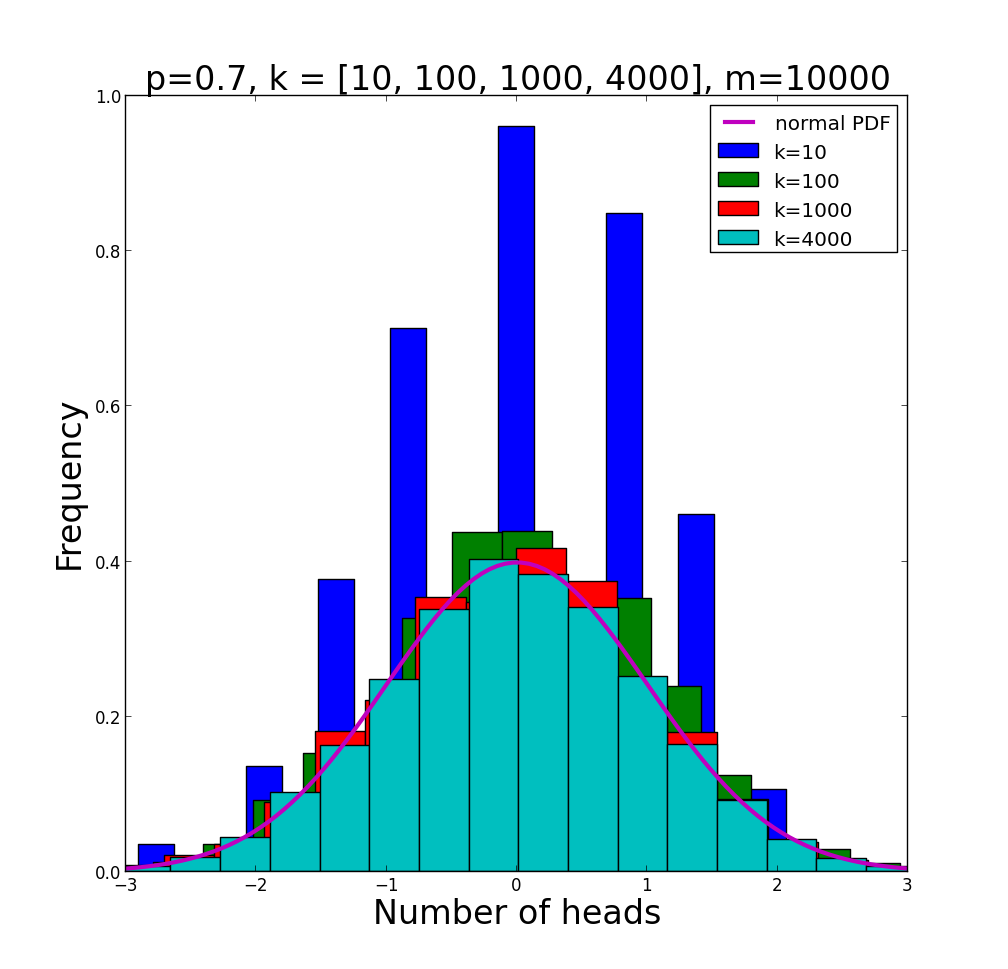
\includegraphics[width=0.45\textwidth]{figs/part_c.png}
%\end{figure}
%}}\fi

\qpart
\item The other interesting pattern that you had seen in the previous
  virtual lab (In particular, in part k of Q1 on HW7) was the
  exponential drop in the frequencies of certain rare events. For an
  exponential drop, the most interesting thing is to understand the
  rate of the exponential --- or the relevant slope on the Log-Linear
  plot.  

  For a coin with probability $p$ of being heads, we are interested in
  the frequency by which tossing $k$ such coins results in more than
  $ak$ heads (where $a$ is a number larger than $p$). We are
  interested in $p=0.3,0.7$ and $a = p+0.05$,
  $p+0.1$.  Take $m = 10000$ and plot the natural log of the frequencies 
  these deviations against $k$ (ranging from 10 to 200). Approximately
  extract the slopes for all 4 of these.

  Compare them in a table against the predictions of the following
  formula (which we will derive later in the course)
  $$D(a||p) = a \ln \frac{a}{p} + (1-a) \ln \frac{1-a}{1-p}.$$
  
  This expression is called the Kullback-Liebler divergence and is also
  called the relative entropy. 

  Finally, add $e^{-D(a||p) k}$ to the plots (there should be 4 of
  these) you have made as straight lines for immediate visual
  comparison. This straight line is called a ``Chernoff Bound'' on the
  probability in question. 

  Comment. 

%\ifsolutions{ \answer { \\
%Suggestions for python students: $m=10,000$ takes a long time to run.  Suggest a lower $m$ at first for faster debugging. To fit a line, you can use "numpy.polyfit(xlist,log(ylist),1)" for a degree 1 polynomial.  There will probably be some 0 values, which will mess up this fitting, so they can replace 0 values with $10^-3$ or something like that.
%\begin{figure}[h!]
%\center
%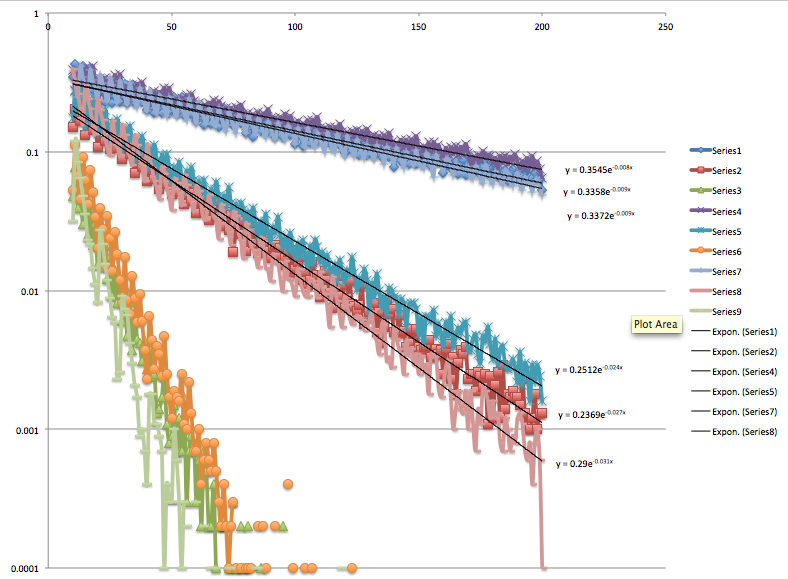
\includegraphics[width=0.65\textwidth]{figs/part_d.png}
%%\caption{1, part d}
%\end{figure}
%}}\fi

\qpart
\item In the previous part, we went directly to one of the most
  powerful bounds we have. A much simpler bound (that we will
  rigorously derive later in the course) is called Chebyshev's
  inequality. For coin tosses, this inequality says 
$$P(|S_k - k p| \geq \epsilon k) \leq \frac{ p (1-p)}{k \epsilon^2}.$$ 

Notice here that Chebyshev's inequality looks at two-sided
deviations. We count both when $S_k$ is much bigger than $kp$ and when
it is much smaller than $kp$. This is the difference from the previous
bounds. 

We can try to use this for the same kind of big deviations that we had
examined above by trying $\epsilon = 0.1, 0.2, 0.3$. Use simulations to
compare what the actual frequency of such deviations is to what
Chebyshev's inequality estimates.  

Try to make an appropriate plot that shows both Chebyshev's
inequality's prediction and where the actual frequencies are? Why is
this hard?

\qpart
\item Lastly, we would like to explore a function that defines how many ways you can choose $k$ distinct objects out of $n$ possible objects. This is written as $\binom{n} {k}$ and is read aloud as ``$n$ choose $k$''. We define $\binom{n}{k} = \frac{n!}{k!(n-k)!}$ So, for example, $\binom{5}{3} = \frac{5!}{3!(5-3)!} = \frac{5\cdot 4 \cdot 3 \cdot 2 \cdot 1}{(3 \cdot 2 \cdot 1) \cdot (2 \cdot 1)} = \frac{120}{12} = 10$. We wish to explore this function. Plot the value $\binom{50}{k}$ on the $y$-axis and $k$ on the $x$-axis for $0 \leq k \leq 50$.
%Let's try plotting this for $n = 4, 10, 25, 50$.
Does this constantly grow as $k$ gets larger? What does the shape of the graph remind you of?
%You should note a defining feature of the graph. 

%\ifsolutions{ \answer { \\
%Suggestions for python students: there is a binomial coefficient function in scipy.  If they don't have scipy, they can use the "math.factorial(n)" and write their own choose function.
%\begin{figure}[h!]
%\center
%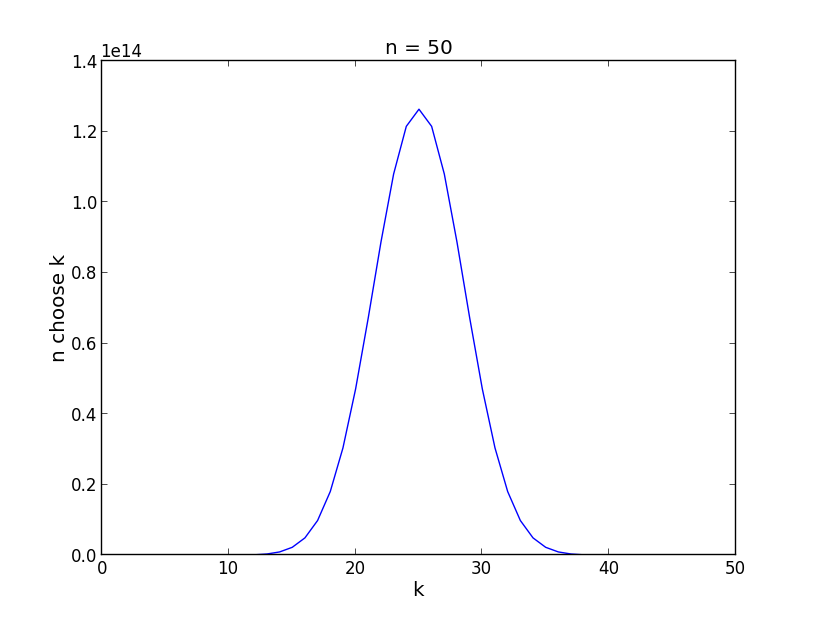
\includegraphics[width=0.5\textwidth]{figs/part_f.png}
%\end{figure}
%}}\fi

\end{enumerate}



\qns{I'm Hungry... How many Pizzas?}

Suppose that a pizzeria lets me choose toppings for the pizza among $10$ different ingredients. I have budget for buying a pizza with $3$ toppings. For this HW, you may express your answers as expressions, rather than as numbers (for example, $\frac{3!}{5!}$ instead of $0.05$).

\begin{enumerate}[a)]
  \qpart 
\item I choose $3$ distinct toppings. If the order in which I order the toppings matters, (for example: ordering Tomatoes, Onions, Mushrooms is different than ordering Tomatoes, Mushrooms, Onions) how many ways are there to order the toppings?

\ifsolutions{ \answer { $10*9*8 = 720$. Because we are sampling without replacement, there are $10*9*8$ different ways to order the toppings. There are $10$ different things to order first, $9$ different things to order second (we can't order the same thing twice) and $8$ things to order third (remember that we can order the first or second topping again).  \\ {\bf Problem Elaboration: } Consider the generalization of this problem, if could order $k$ toppings ($k \leq n$), we would have $\frac{n!}{(n-k)!}$ possible orders. If we were allowed to order the same topping multiple times we would have $10^k$ different orders (since there would always be $10$ choices for the first, second, third, etc. topping).

}}\fi
  
  \qpart
\item Now I realize that it doesn't matter what order I ask for the toppings, I still get the same pizza. Again using $3$ distinct toppings out of a possible $10$, how many different types of Pizza can I order?

\ifsolutions{ \answer { 
$\binom{10}{3} = 120$. Again, this is read aloud as "$10$ choose $3$. This number represents the number of ways to select $3$ unique items out of a possible of $10$ unique items. By definition, $\binom{10}{3} = \frac{10!}{(10-3)!3!}$ \\ {\bf Problem Elaboration: } Let us briefly walk through the derivation of $\binom{n}{k}$. We see that from the previous problem there are $10*9*8 = \frac{10!}{(10-3)!}$. Take a moment to see why this is true (a lot of terms cancel out). We realize that with the number $ \frac{10!}{(10-3)!}$ we are counting each order multiple times. For example, we count the "Tomatoes, Mushrooms, Onions" and "Tomatoes, Onions, Mushrooms" and "Mushrooms, Onions, Tomatoes", etc. all as different orders when in fact they are the same order. So we wish to realize how many times we are counting each order. So how many ways are there to arrange "Mushrooms, Onions, Tomatoes?" Well, there are $3$ items to arrange so we have $3$ choices for the first thing we order, $2$ for the second order, and $1$ for the first. So we have $3!$ ways to order the same unordered set of three toppings. This means each topping is getting counted $3!$ times when we really should count it once. So we have \\$(\text{Number of 3-topping pizzas when order matters}) = 3! * (\text{Number of 3-topping pizzas when order does not matter})$. Therefore we have \\$ \text{(Number of 3-topping pizzas when order does not matter)} = (\text{Number of 3-topping pizzas when order matters})/{3!} \\ \text{(Number of 3-topping pizzas when order does not matter)} = \frac{10!}{(10-3)!} / 3! = \frac{10!}{(10-3)!3!} = \binom{10}{3} $

}}\fi

  \qpart
\item I don't have to get $3$ toppings. If I can instead choose 0, 1, 2, or 3 distinct toppings. For example I could order tomatoes and onions and no third topping. How many different pizzas can I order now?

\ifsolutions{ \answer {  This answer follows from the work in the previous answer. We now add up the number of ways to order $3$ unique toppings, $2$ unique toppings, $1$ unique topping, and $0$ unique toppings.
$\binom{10}{3} + \binom{10}{2} + \binom{10}{1} + \binom{10}{0} = 176$. Please note that $0! = 1$ and therefore $\binom{10}{0} = 1$. In general, it is easy enough to prove that $\binom{n}{0} = 1$ and $\binom{n}{1} = n$.  These identities pop intuitively when you consider reading it as "$n$ choose $1$." How many ways are there to \underline{choose} $1$ item out of $n$ items? Clearly the answer is $n$, or $\binom{n}{1}$.

}}\fi

  \qpart
\item The waiter informs me that I can order repeat toppings (put 2 or 3 portions of the same topping). So now I can order Tomatoes, tomatoes, and onions, for example. Still sticking with my same budget, how many different pizzas can I order, making sure I order exactly $3$ toppings total (although the toppings may not be distinct).

\ifsolutions{ \answer { This answer is a little tricky. We decide to sum over the number of unique toppings we order. We realize we can order $3$, $2$, or $1$ unique topping (we can't order $0$ unique toppings because we have to order exactly $3$ toppings total). \begin{itemize}
\item If we order $3$ unique toppings, then this is the same problem as part b. Therefore we have $\binom{10}{3}$.
\item if we order $2$ unique toppings, then we $2*\binom{10}{2}$ pizzas. Why? Well first, we select the number of ways we can \underline{choose} $2$ different toppings which is $\binom{10}{2}$. We realize that once we have chosen our $2$ toppings (for example, "onions and mushrooms" we have $2$ choices for which topping we want to double (we can order "onions, onions, mushrooms" or "onions, mushrooms, mushrooms"). 
\item if we order $1$ unique topping, then we have to order $3$ portions of that topping, so we simply \underline{choose} one topping to order. Therefore we have $\binom{10}{1}$.
\end{itemize}  
Thus our final answer is $\binom{10}{3} + 2*\binom{10}{2} + \binom{10}{1} = 220$

}}\fi

\qpart
\item Using the same framework where I can get repeated topping, and not restricting myself to exactly 3 toppings, how many pizzas can I order?

\ifsolutions{ \answer { We approach this solution using a similar idea from the last problem. We separately add the number of pizzas we can order with $i$ unique toppings for $i \in {0,1,2,3}$. \begin{itemize}
\item If we order $3$ unique toppings, then this is the same problem as part b. Therefore we have $\binom{10}{3}$.
\item If we order $2$ unique toppings we have (number of choices for $2$ toppings)*(choice for doubling a topping or not doubling). In other words, once we pick one of the $\binom{10}{2}$ toppings, we have $3$ more choices: we can double the first topping, we can double the second topping, or we can double neither topping. Therefore we have $3*\binom{10}{2}$
\item If we order $1$ unique toppings, we still have $3$ more choices. We either order one, two, or three servings of the toppings. Therefore we have $3*\binom{10}{1}$
\item There is only one pizza we can order if we choose $0$ toppings, so $\binom{10}{0}$
\end{itemize}
Thus our final answer is $\binom{10}{3} + 3*\binom{10}{2} + 3*\binom{10}{1} +\binom{10}{0} = 286$

}}\fi
 
\qpart
\item I go to a cheaper pizzeria, I can now order up to $5$ toppings. How many  pizzas can I buy? (Using the same rules as e above).

\ifsolutions{ \answer { We approach this solution using a similar idea from the last problem. We separately add the number of pizzas we can order with $i$ unique toppings for $i \in {0,1,2,3,4,5}$. \begin{itemize}
\item If we order $5$ unique toppings, once we choose our $5$ toppings we have no choices left to make regarding ordering multiple servings of a topping. Therefore we have $\binom{10}{5}$ pizzas.
\item If we order $4$ toppings, once we select which $\binom{10}{4}$ toppings we still have many choices. We must choose which of the $4$ toppings to double (which is $\binom{4}{1}$ choices), or we may choose to not double any topping (which is just $1$ choice). Therefore we have $\binom{10}{4}* (\binom{4}{1} + 1)$.
\item If we order $3$ toppings, once we select which $\binom{10}{3}$ toppings we still have many choices. We can choose to triple one topping, and we have $\binom{3}{1}$ toppings to choose to triple. We can choose to double one topping, and we have $\binom{3}{1}$ toppings to choose to double. We may choose to double two toppings, in which case we can choose $\binom{3}{2}$ different toppings to double. Lastly, we may choose to simply order exactly $3$ servings, which is only one choice. Therefore we have $\binom{10}{3} * (1 + 2*\binom{3}{1} + \binom{3}{2})$
\item If we order $2$ toppings, once we select which $\binom{10}{2}$ toppings we still have many choices: \begin{itemize} \item We can choose to quadruple one of the toppings, and we have $\binom{2}{1}$ toppings to choose to quadruple. 
\item We can choose to triple one topping and double another. We then have $\binom{2}{1}*\binom{1}{1} = \binom{2}{1}$ ways to choose those toppings. 
\item We can choose to only triple one topping, in which case we have $\binom{2}{1}$ choices. 
\item We can choose to double both of the toppings, this gives us $\binom{2}{2} = 1$ choices. 
\item we can choose to double only one of the toppings, giving us $\binom{2}{1}$ choices. 
\item Lastly, we may choose to only order $1$ serving of each topping, giving us $\binom{2}{0} = 1$ choices \end{itemize}
 Therefore we have $\binom{10}{2} * (2 + 4*\binom{2}{1} )$
\item If we order $1$ topping, once we select which $\binom{10}{1}$ topping we can choose to get either $1$, $2$, $3$, $4$, or $5$ servings of it. This counts for a total of $\binom{10}{1}*5$ pizzas. 
\item Lastly, we may order $1$ zero topping pizza.
\end{itemize}
Overall, our answer is
$$\binom{10}{5} \ + \ \binom{10}{4}* (\binom{4}{1} + 1) \ + \ \binom{10}{3} * (1 + 2*\binom{3}{1} + \binom{3}{2}) \ + \binom{10}{2} * (2 + 4*\binom{2}{1} )\  + \ \binom{10}{1}*5$$
$$= \binom{10}{5} \ + \ \binom{10}{4}*5 \ + \ \binom{10}{3} * (1 + 2*3 + 3) \ + \binom{10}{2} * (2 + 4*2 )\  + \ \binom{10}{1}*5$$
$$= \binom{10}{5} \ + \ \binom{10}{4}*5 \ + \ \binom{10}{3} *10 \ + \binom{10}{2} *10\  + \ \binom{10}{1}*5$$ $$=3002$$


%An alternate form of this would be
%
%$$\binom{10}{5} \ + \ \binom{10}{4}* (\binom{4}{1} + \binom{4}{0}) \ + \ \binom{10}{3} * (\binom{3}{2} + 2*\binom{3}{1} + \binom{3}{0}) \ + \ \binom{10}{2} * (\binom{4}{1} + \binom{3}{1} +\binom{2}{1} + \binom{1}{1}) \ + \ \binom{10}{1}(5) $$






As a challenge problem, can you give the answer to f if we can order up to $k$ toppings from $n$ choices?

}}\fi

\end{enumerate}

\ifmotivation
{\motivation {Motivation - Counting continued but d) is tricky.}}
\fi 


%\qns{Include the stars, exclude the bars}
%
%You are packing for a hike, and you have to choose what to bring with you. You can pick from energy bars, lemons, and bananas. You do not
%want your backpack to be too heavy, so you decide to bring exactly $12$ items with you.
%
%\begin{enumerate}
%  \qpart
%  \item If you have an unlimited supply of each item, in how many ways can you pack your backpack?
%  \qpart
%  \item Now assume that you have $5$ energy bars, $3$ lemons, and $3$ bananas. Now in how many ways can you pack your backpack?
%\end{enumerate}


\qns{Hunger Games}

In this modified version of the book (and movie), Esther is a young adult eligible for tribute to the Hunger Games. Esther is asked to pick 5 cards from a total of 100. Out of these 100 cards, 10 are marked. If at least 1 of the cards out of the 5 Esther picked is a marked card, Esther will go on as tribute to the Hunger Games. 

\begin{enumerate}[a)]
  \qpart
\item How many ways in total are there for Esther to pick 5 out of 100 cards? The order in which she picks these cards does not matter. 

\ifsolutions{ \answer {
$\binom{100}{5}$. Again, we read this answer aloud as "$100$ choose $5$." This is equivalent to $\frac{100*99*98*97*96}{5!} = \frac{100!}{5!(100-5)!}$. We can see this derived since we have $100$ choices for the first card, and the second card can be anything but the first card, so we have $99$ choices for the second card, and so on. We have to divide by $5!$ since every combination of $5$ cards has $5!$ permutations. In other words, there are $5!$ to arrange each set of $5$ cards, so we are over counting by a factor of $5!$ Thus, we must divide $10*9*8*7*6$ by $5!$. In the future, you can read this answer and immediately see it as a form of "$n$ choose $k$" and can write $\binom{100}{5}$ immediately.

}}\fi
  
  \qpart
\item How many ways can Esther choose the 5 cards such that all are unmarked? Now what is the probability that she will not go on to the Hunger Games? 

\ifsolutions{ \answer {
To answer the first question, we count all the ways to pick $5$ cards from all the unmarked cards. According to the question there are $90$ unmarked cards. Therefore there are $\binom{90}{5}$ ways to pick all unmarked cards and thus $\binom{90}{5}$ ways to avoid going on the Hunger games. We use the rule that since each outcome is equally likely, to calculate the probability she will not go to the hunger games we count the outcomes in which she will not go to the hunger games ($\binom{90}{5}$) and divide by the total number of outcomes ($\binom{100}{5}$). Therefore our answer is $\frac{\binom{90}{5}}{\binom{100}{5}} \approx 0.58$
}} \fi
  
  \qpart
\item What is the probability that she chooses 5 cards such that 1 is marked and the rest are unmarked? How about the configuration where 2 cards are marked and the rest are unmarked? 
  
\ifsolutions{ \answer {
In order to compute this probability, we need to count the number of outcomes that have $1$ marked card and the $4$ unmarked. Then we have to calculate the number of outcomes that have $2$ marked cards and the $3$ unmarked.
\begin{itemize}
\item Without loss of generality, we can imagine the first card pulled is the marked card. (This is safe to do because we don't consider the order as important. All the outcomes have $1$ marked card, so we just think of this card as being pulled first). we first count the number of ways to choose the $1$ marked card. This happens $\binom{10}{1}$ choices. The rest of the $4$ cards there are $90$ choices for the second card (it must not be marked), and $89$ choices for the third card (it must not be marked, and it cannot be the same as the first card). Then $87$ and $86$ choices for the next two cards. However, we are double counting by a factor of $4!$ Since this way of counting does not ignore order So, we have $10*\frac{90*89*88*87}{4!}$. We can think of this answer happening another way, we have $\binom{10}{1}$ choices for the marked card, and to \underline{choose} $4$ unmarked cards out of $90$ unmarked cards we have $\binom{90}{4}$. Therefore our answer can be written as $\binom{10}{1}*\binom{90}{4}$. Then the probability of this occurring is $\frac{\binom{10}{1}*\binom{90}{4}}{\binom{100}{5}} \approx 0.34$. 
\item Now using the insight from the previous step, we can easily solve this problem. We have to \underline{choose} $2$ marked cards out of the $10$ marked cards, and we have to \underline{choose} $3$ unmarked cards out of the $90$ unmarked cards. We get $\binom{10}{2}*\binom{90}{3}$. Therefore the probability of this occurring is $\frac{\binom{10}{2}*\binom{90}{3}}{\binom{100}{5}} \approx 0.07$
\end{itemize}
}} \fi  
  
  \qpart
\item What is the probability that Esther will go on to the Hunger Games? 
  
\ifsolutions{ \answer {
We can calculate this one of two ways. First, we know that since probabilities have to sum to $1$, we know that the \\ (Probability that Esther goes to hunger games) + (Probability Esther does not) = 1 \\ and therefore Probability Esther does not = 1 - (answer to part b) $\approx 0.42$ Let us derive this another way. The probability that she will go to the hunger games can be computed by calculated all the outcomes in which she goes to the hunger games, she chooses $1$, $2$, $3$, $4$, or $5$ marked cards. \\ Therefore this happens in $\binom{10}{1}*\binom{90}{4} + \binom{10}{2}*\binom{90}{3} + \binom{10}{3}*\binom{90}{2} + \binom{10}{4}*\binom{90}{1} + \binom{10}{5}*\binom{90}{0}$ outcomes. Recall that $\binom{n}{0} = 1$. So our answer is \\ $\frac{\binom{10}{1}*\binom{90}{4} + \binom{10}{2}*\binom{90}{3} + \binom{10}{3}*\binom{90}{2} + \binom{10}{4}*\binom{90}{1} + \binom{10}{5}*\binom{90}{0}}{\binom{100}{5}} \approx 0.42$ 
}} \fi  
  
  \qpart
\item Given that Esther picked 1 marked card and 4 unmarked cards (she is going to the Hunger Games), her friend Tommy is now forced to choose 5 cards from the remaining pile. Calculate the probability that he will go to the Hunger Games. 

\ifsolutions{ \answer {
Since Esther has picked $5$ cards, there are only $95$ cards left. This means that there are a total of $\binom{95}{5}$ possible hands (combinations of cards) to pull. There are now only $4$ marked cards and $86$ unmarked cards. Therefore the probability Tommy does not go to the hunger games can be calculated by counting the outcomes in which he \underline{chooses} $5$ unmarked cards out of the $95$ remaining cards. Therefore the probability is $\frac{\binom{86}{5}}{\binom{95}{5}} \approx 0.60$
}} \fi

\end{enumerate}



\ifmotivation
{\motivation {Motivation - Basic counting and probability.}}
\fi 

\qns{Clinical Trials}

You are creating a test for a rare disease that only 1 in 1000 people have. If a person has the disease, there is a 95\% chance that your test will be positive.  But if the person does not have the disease, there is only an 85\% chance the test will be negative.

\begin{enumerate}
\qpart 
\item[a)] Let $D$ be the event that you have the disease, and $H$ be the event that you are healthy.  Let $A$ be the event that the test comes out positive, and $B$ be the event that it comes out negative.  Write an expression for $\mathbb{P}(D|A)$ (the probability you have the disease given a positive test result) in terms of the probabilities given above.  Plug in the given probabilities into your expression and calculate the numerical value of $\mathbb{P}(D|A)$.

\ifsolutions{ \answer { We know from Bayes rule that
\[ P(D|A) = \frac{P(D)P(A|D)}{P(A)}. \]

We know that $P(D) = 0.001$ and $P(A|D) = 0.95$, but it is unclear how to compute $P(A)$. However, we do know that the probability of a positive test result should be the probability of a positive test result and disease, plus the probability of a positive test result and healthy. This gives us
\[ P(A) = P(A,D) + P(A,H) = P(D)P(A|D) + P(H)P(A|H). \]

which we have expanded above using Bayes rule.  Now we have $P(A)$ in term of quantities we know, and can write
\[ P(D|A) = \frac{P(D)P(A|D)}{P(D)P(A|D) + P(H)P(A|H)} = \frac{0.001 \cdot 0.95}{0.001 \cdot 0.95+ 0.999 \cdot 0.15} = 0.62997\%, \]

so even given a positive test result, we get a very very small probability of disease.
}}\fi

\qpart
\item[b)] Write an expression for $\mathbb{P}(H|B)$, the probability you are healthy given a negative test result.  Evaluate the numerical result of this expression as well.

\ifsolutions{ \answer { Similarly, we get
\[ P(H|B) = \frac{P(H)P(B|H)}{P(B)} = \frac{P(H)P(B|H)}{P(H)P(B|H) + P(D)P(B|D)} = \frac{0.999 \cdot 0.85}{0.999 \cdot 0.85 + 0.001 \cdot 0.05} = 99.9941\%. \]
}}\fi

\qpart
\item[c)] For your test to gain approval, the chance of disease given a positive test result must be above 90\%. What would the accuracy of the test have to be to ensure this result?  (You may now assume the accuracy of the test is the same whether you have the disease or not.)

\ifsolutions{ \answer {
Solve for $x$:
\[ P(D|A) = \frac{0.001 \cdot x}{0.001 \cdot x + 0.999 \cdot (1-x)} = 0.9 \quad \Rightarrow \quad x = 99.9889\% \]
}}\fi

\end{enumerate}

%\qns{Hunger Games Part 2}
%
%In this again modified version of the book (and the movie), the world is divided into 12 districts, namely District 1 through District 12, and the Capitol. The districts are the colonies of the Capitol, which is run by an evil leader President Snow. The districts have begun to revolt. Powerful President Snow has 20 divisions of indistinguishable robot soldiers. 
%
%\begin{enumerate}[a)]
%  \qpart
%\item How many ways are there for President Snow to send the divisions such that each district has at least 1 division of soldiers?
%  
%  \qpart
%\item Now, President Snow also has a choice to send 0 divisions to districts that do not need soldiers. How many total ways are there for President Snow to divide the 20 divisions?  Sending all 20 divisions to District 1 is different from sending all to District 12. (Hint: represent the distinct outcomes using binary strings. How many of these binary strings are there?)
%\end{enumerate}
%
%\ifmotivation
%{\motivation {Motivation - Stars and Bars problem.}}
%\fi    






\qns{Write your own problem} \\
Write your own problem related to this week's material and solve it. You may still work in groups to brainstorm problems, but each student should submit a unique problem. What is the problem? How to formulate it? How to solve it? What is the solution?

\qns{Midterm question 3} \\
Re-do midterm question 3.
\qns{Midterm question 4} \\
Re-do midterm question 4.
\qns{Midterm question 5} \\
Re-do midterm question 5.
\qns{Midterm question 6} \\
Re-do midterm question 6.
\qns{Midterm question 7} \\
Re-do midterm question 7.
\qns{Midterm question 8} \\
Re-do midterm question 8.
\qns{Midterm question 9} \\
Re-do midterm question 9.
\qns{Midterm question 10} \\
Re-do midterm question 10.
\qns{Midterm question 11} \\
Re-do midterm question 11.
\qns{Midterm question 12} \\
Re-do midterm question 12.
\qns{Midterm question 13} \\
Re-do midterm question 13.
\qns{Midterm question 14} \\
Re-do midterm question 14.
  
  
    
\end{qunlist}


\end{document}
